\documentclass{article}
\usepackage{biblatex}
\usepackage{graphicx}
\usepackage[margin=1in]{geometry}
%\usepackage{amsmath}
\usepackage{parskip}
\begin{document}
\title{16-831 Project 3: Robot Localization}
\author{Alex Brinkman, Shivam Gautam, Tushar Agrawal}
\maketitle

\begin{figure}[!h]
    \centering
    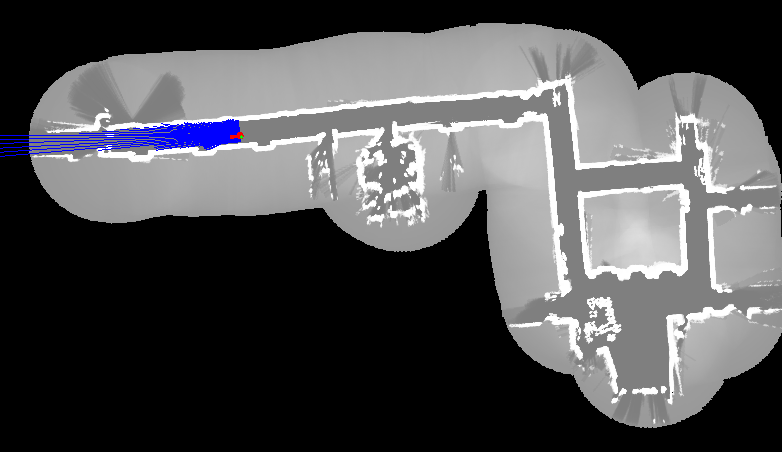
\includegraphics[width=4.0in]{media/graphics_example.png}
    \caption{Visualization of the Particle Filter after Convergence}
\label{fig:1}
\end{figure}

\section{Approach}
    We started by first developing the modules in isolation to facilitate future integration. We started by independently developing the sensor model, motion model, ray tracing, and graphics engine, and log-streaming modules first. We performed unit testing on each to verify they were working properly, relying heavily on the graphics to validate the complex modules. Once the modules were build up, we integrated the modules and debugged the interfacing issues and added importance resampling. Since the modules were tested independently, this was relatively painless. Finally, we refined the pipeline to improve runtime and tuned the particle filter parameters to find a good trade-off between convergence speed and correctness. Figure \ref{fig:1} depicts the final outcome of the particle filter.

\section{Implementation}
    We implemented the particle filter in C++ and used a private git repo in our workflow.  All modules were implemented as stand alone classes and invoked in executable scripts.  The final integration took the individual classes and encapsulated the modules while exposing configuration parameters to ease tuning. We used GNUplot-iostream to visualize 1D data like the sensor model and the SFML library to visualize the map, particles, and laser readings.  

\subsection{Sensor Model}
    The sensor model consists of a superposition of an exponential decay function, Gaussian distribution, uniform distribution, and max value.  The Gaussian distribution mean is placed at the expected range measurement with a tunable variance. Since the we need to sum the log-likelihood of each of the 180 range readings, the uniform distribution of the model is 1 so for any range measurement this provides a non-negative log-likelihood. The decay function plays a small role in the overall shape of the function, only affecting the first meter or so. The Gaussian was tuned first by using reasonable values for gain factor and standard deviation.  We found that once we set the initial values to something reasonable, we did not have to tune this model much to get the performance we desired. Figure \ref{fig:2} shows the final sensor model used in our tuned model and Figure \ref{fig:3} shows the final parameters.
\begin{figure}[!h]
    \centering
    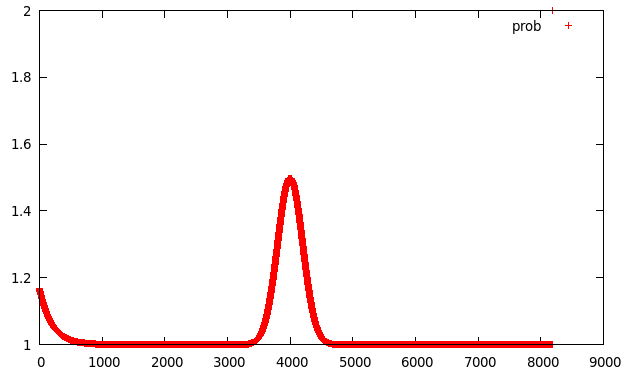
\includegraphics[width=2.5in]{media/sensor_model.png}
    \caption{Sensor Model for reference reading for 4000cm, X-axis is cm}
\label{fig:2}
\end{figure}

\begin{figure}[!h]
    \centering
    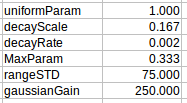
\includegraphics[width=2.0in]{media/sensor_model_parameters.png}
    \caption{Final Sensor Model Parameters}
\label{fig:3}
\end{figure}

\subsection{Motion Model}

Using the odometry readings from the log, the particle position was updated from the measurements augmented by some Gaussian noise. The motion of the particle between two consecutive odometry readings was broken down into three motions - 
\begin{itemize}
\item A rotation to align the heading with the axis of translation.
\item A translation to reach the final x,y position.
\item A final rotation at the x,y postition to align the heading with the final heading.
\end{itemize}

The particles were propagated based on the the variance associated with the rotation and translation. The description of the noise parameters used for the motion model were as follows[1] - 
\begin{itemize}
\item alpha1: Specifies the expected noise in odometry's rotation estimate from the rotational component of the robot's motion. 
\item alpha2: Specifies the expected noise in odometry's rotation estimate from translational component of the robot's motion. 
\item alpha3: Specifies the expected noise in odometry's translation estimate from the translational component of the robot's motion. 
\item alpha4: Specifies the expected noise in odometry's translation estimate from the rotational component of the robot's motion. 
\end{itemize}

\begin{figure}[!h]
    \centering
    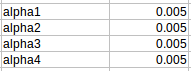
\includegraphics[width=2.0in]{media/motion_model_parameters.png}
    \caption{Final Motion Model Parameters}
\label{fig:4}
\end{figure}

\subsection{Ray Tracing}

Ray tracing was needed to compute the predicted range readings for a given particle.  For each angle -90 to 90 degrees about the heading angle, a ray was cast out from the particle through the map grid and terminated when it hit the edge of the map.  Figure \ref{fig:5} Shows a comparison between predicted ranges compared to the replayed laser readings. This visualization was part of the verification testing of this module.

\begin{figure}[!h]
    \centering
    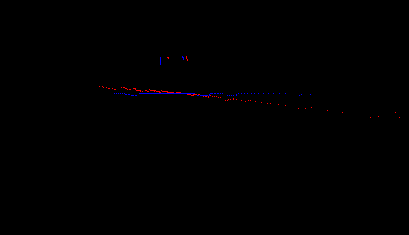
\includegraphics[width=2.5in]{media/ray_tracing.png}
    \caption{Ray Tracing(Red) Validation against Logged Data(Blue)}
\label{fig:5}
\end{figure}

Since ray casting was required for each particle, 180 degrees, up to a max distance of ~800 grid elements for each iteration, it was the part we were most concerned about affecting runtime.  We decided to implement a caching scheme that would memorize ray traced results and greatly reduce repeated computation. We discretized the number of angles to 360 degrees for each of the points on the grid. We could allow the system to lazily compute the ray traced table but ended up implementing the precomputation for every point in free space before running the localization algorithm.   

\subsection{Importance Resampling}

After a laser reading update, each particle was assigned a weight according to how well it fit the sensor reading. Our implementation used low variance resampling. We used the algorithm laid out by Cyrill Stachniss from his lectures[2].  This technique forces a set of samples to be sampled randomly but at small, regular intervals through the particle weights. This ensures that some particles of low weight still survive and ensures the filter will not converge when the weights are uniform i.e. when no information is gained from the laser reading.  This has the added benefit of running in linear time.

\section{Results}

Our particle filter algorithm converges to an accurate solution when using 3000 particles and the filter parameters described above on all provided data logs.  Including visualizations, we get approximately 17 updates per seconds running on a single core of a 4.0 Ghz Intel i7-4790K processor. This performance was deemed acceptable even without parallelization.

\section{Future Work}

There are several obvious areas to improve our particle filter.  The first is parallelization. We could approximately achieve a speed up of approximately Nx using N threads given the particle propagations computations are inherently parallel operations.


\section{Kidnapped Robot Problem}

We implemented a basic solution for the kidnapped robot problem and tested its working on a ``kidnap.log'' file which was created by merging data from two different log files (robotdata1.log and robotdata3.log). \\
In this solution, the system detects if the sum of weights of all particles in an iteration drops by certain factor compared to the previous iteration, then the robot is considered to be ``kidnapped''. This ``kidnapped'' factor is tunable and currently set to 0.82. In such a scenario, the current particles are cleared and a new random set of particles are reinitialized and the system reconverges to the new position of the robot. A video depicting a run on the kidnapped robot problem is also included.

\section{Adaptive number of particles}

In the current implementation only a fixed number of particles was used due to lack of time for the implementation. We considered the approach of likelihood-based sampling which is relatively easy to implement. \\
Likelihood-based adaptation determines the number of samples such that the sum of non-normalized likelihoods (importance weights) exceeds a prespecified threshold. Intuitively, if the sample set is well in tune with the sensor reading, each individual importance weight is large and the sample set should remain small. If, however, the sensor reading carries a lot of surprise, as is the case when the robot is globally uncertain or when it lost track of its position, the individual sample weights are small and the sample set should become large. The likelihood-based adaptation directly relates to the property that the variance of the importance sampler is a function of the mismatch between the proposal distribution and the distribution that is being approximated. \\
In the presence of more time, the KLD sampling approch could be implemented for updating the number of particles adaptively.


\section{References}\
[1] http://wiki.ros.org/amcl 

[2] Cyrill Stachniss,  https://www.youtube.com/watch?v=eAqAFSrTGGY

[3] Dieter Fox, ``KLD-Sampling: Adaptive Particle Filters''

\end{document}